\documentclass{article}
\usepackage{minted}
\usepackage[T1]{fontenc}
\usepackage{polski}
\usepackage[utf8]{inputenc}
\usepackage[polish]{babel}
\usepackage[parfill]{parskip}
\usepackage[a4paper, total={6in, 8in}]{geometry}
\usepackage{graphicx}
\graphicspath{ {./images/} }

\title{System zarządzania partią polityczną - dokumentacja}
\author{Patryk Kumor}


\begin{document}
  \maketitle
  \newpage
  \tableofcontents
  \newpage


\section{Potrzebne pakiety i uruchomienie programu}

\subsection{ Potrzebne pakiety } 

Program został napisany w Pythonie 2.7, z użyciem następujących bibliotek: 
\begin{itemize}
    \item argparse 
    \item json 
    \item sys 
    \item psycopg2 
\end{itemize}
Wszystkie powyższe moduły, oprócz ostatniego - psycopg2 - powinny być dostarczone wraz z podstawową dystrybucją pythona. \newline
Aby zainstalować psycopg2 należy skorzystać z PIP - package managera do\,języka python, w tym celu należy wykonać polecenie:
\begin{minted}{shell}
    \$ pip install psycopg2
\end{minted}

\subsection{ Uruchomienie programu }  
Program do zarządzania partią przyjmuje na wejściu obiekty json, które są odczytywane jako ciąg wywołań funkcji API. \newline
Program rozróżnia kilka typów wywołań: 

\paragraph{}  
Aby wywołać program z odczytem linii zawierających obiekty json (jeden obiekt na linię) ze\,\,standar-dowego wejścia w pętli:
\begin{itemize}
\item dla pierwszego wywołania wraz z flagą init:
\begin{minted}{shell}
    \$ python main.py --init
\end{minted}
\item dla kolejnych wowołań:
\begin{minted}{shell}
    \$ python main.py 
\end{minted}
\end{itemize}

\paragraph{}  
Aby wywołać program wraz z odczytem standardowego wejścia zawartego w pliku (każda linia w\,\,pliku jest obiektem json):
\begin{itemize}
\item dla pierwszego wywołania wraz z flagą init:
\begin{minted}{shell}
    \$ python main.py --init < <input_file>
\end{minted}
\item dla kolejnych wowołań:
\begin{minted}{shell}
    \$ python main.py < <input_file>
\end{minted}
\end{itemize}

\paragraph{}  
Aby wywołać program wraz z odczytem zawartości pliku podanego jako argument (każda linia w\,pliku jest obiektem json) należy użyć flagi -\,-f \newline
(Program po skończoeniu odczytywania zawartości pliku przechodzi w tryb ciągłego czytania standardowego wejścia)
\begin{itemize}
\item dla pierwszego wywołania wraz z flagą init:
\begin{minted}{shell}
    \$ python main.py --init --f <input_file>
\end{minted}
\item dla kolejnych wowołań:
\begin{minted}{shell}
    \$ python main.py --f <input_file>
\end{minted}
\end{itemize}

\paragraph{Zakończenie pracy programu \newline}  
Program kończy się automatycznie w przypadku odczytywania standardowego wejścia za pomocą\,\textbf{<},
w przypadku ciągłego odczytywania kolejnych linii program zakończy się gdy zostanie użyty skrót \textbf{ctrl+c}













\newpage
\section{Model fizyczny}
Program przy swoim pierwszym uruchomieniu (wraz z argumentem -\,-init) po pomyślnym połączeniu z bazą danych
tworzy w niej wszystkie potrzebne mu elementy, które są przedstawione na poniższym rysunku. \newline
(Cały schemat użyty podczas tworzenia zawartości bazy danych zawarty jest w pliku \textbf{base.sql})
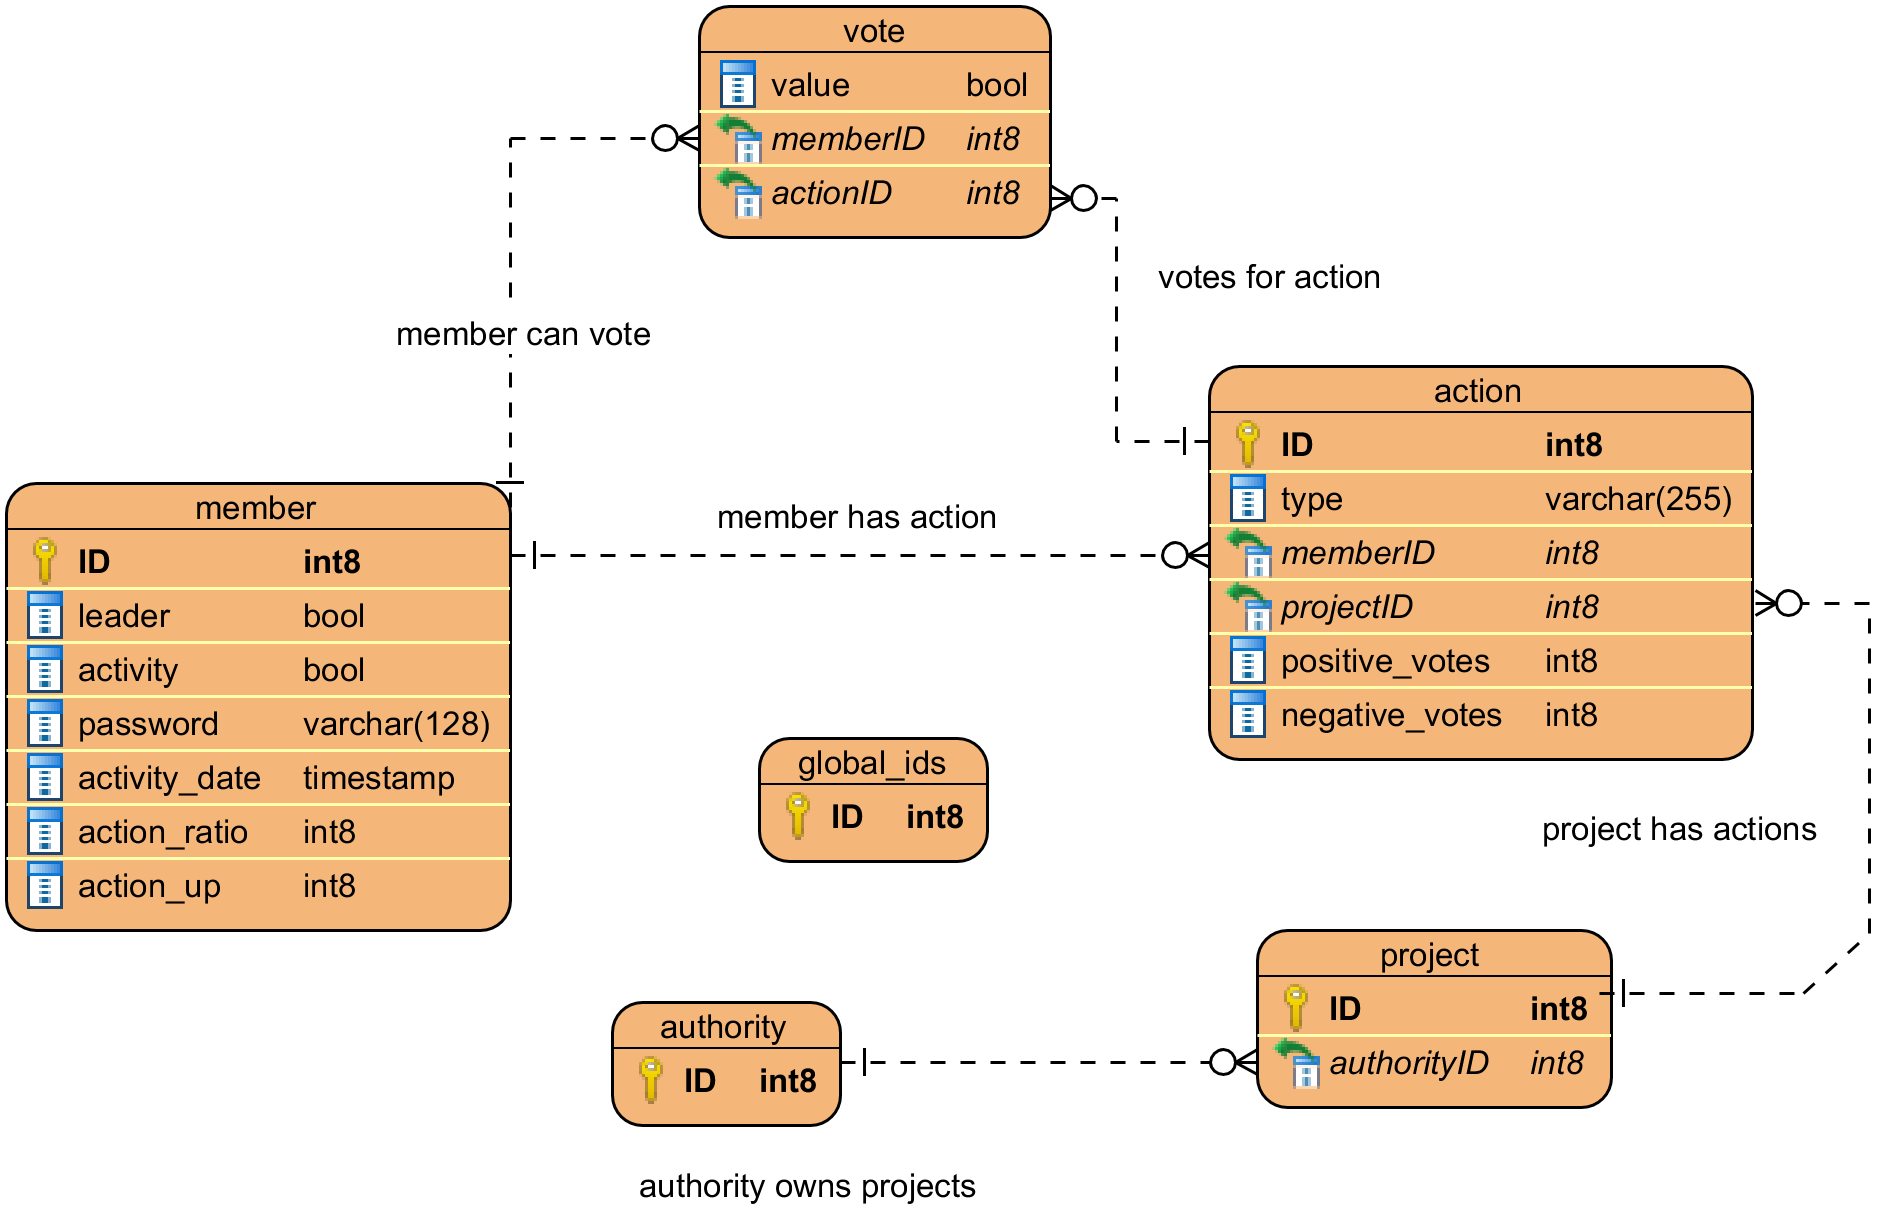
\includegraphics[scale=0.303]{base}  \newline
Użytkownik init, za pomocą którego łączymy się z bazą, posiada wszystkie uprawnienia potrzebne w programie w tym musi mieć uprawienia do: CREATE TABLE, ADD CONSTRAINT, CREATE user, GRANT {przywilej}.
Użytkownik init również tworzy nową rolę \textbf{app} z uprawieniami UPDATE, INSERT i SELECT na powyższych tabelach \newline  \newline 
Tabela\textbf{ global\_ids} przechowuje wszystkie id, które zostały użyte do tej pory w programie, dzięki temu jesteśmy w stanie kontrolować globalną unikalność id we wszystkich tabelach \newline
Wytłumaczenie zawartości kolumn, które mogą być niejasne:
\begin{itemize}
\item value w \textbf{vote} - przechowuje informację o tym czy oddany głos jest za (True) czy przeciw (False)
\item positive\_votes i negative\_votes w \textbf{action} - przechowuje informację o oddanej sumarycznej liczbie głosów za/przeciw wobec danej akcji
\item action\_up w \textbf{member} - przechowuje wartość wszystkich głosów upvotes wobec projektów które dany członek utworzył
\item action\_ratio w \textbf{member}- przechowuje wartość (downvotes - upvotes), która potrzebna jest do uznania członka za trolla (jeśli jest dodatnia)
\end{itemize}







\newpage
\section{Implementacja}




\subsection{Dokładny opis wejścia } 
Obiekty json podawane na wejściu mają strukturę: 
\begin{minted}{js}
{     
    <function> : <value>        // nazwa funkcji 
    {
        <arg1> : <value>        // argumenty funkcji
        <arg2>  : <value> 
        . . . 
        <argn>  : <value> 
    }
}
\end{minted}
Na przykład funkcja \textbf{open} z argumentami \textbf{<database>} \textbf{<login>} oraz \textbf{<password>} może zostać przekazana na wejściu jako:
\begin{minted}{js}
{ "open": { "database": "student", "login": "app", "password": "qwerty"}}
\end{minted}
Skutkuje to wywołaniem przez program odpowiedniej funkcji przetwarzającej taki obiekt (mającej na celu ustanowienie połączenia z bazą danych wraz z danymi dostępowymi podanymi w argumentach)




\subsection{INIT i kolejne wywołania programu}
Podczas pierwszego uruchomienia programu należy użyć flagi -\,-init.
Podczas uruchomienia -\,-init program pobiera wyłącznie jsony z funkcją open i leader.
Jako pierwszy json pobrany powinien być ten zawierający <open> który definiuje elementy bazy i nawiązuje z nią połączenie,
w przypadku niepowodzenia funkcji obsługującej <open> program zakończy działanie. \newline
Kolejne wywoałania funkcji obsługującej <leader> będą definiować nowe krotki członków, którzy są leaderami. 

Kolejne wywołania programu (bez flagi -\,-init) pobierają i obsługują tylko jsony z funkcjami: 
open, support/protest, upvote/downvote, actions, projects, votes i trolls, 
które zostaną szczegółowo opisane w dalszej części dokumentacji.
Również tutaj w przypadku niepowodzenia <open> program zakończy pracę.  

Program przetwarza wejście parserem json, po czym przekazuje je do funkcji \textbf{if\_case(dic, case)}, 
której argumentem jest nowo utworzony słownik powstały na wskutek działania parsera, oraz nazwa funkcji zawarta w jsonie

W dalszej części dokumentacji opisane będą sposoby działania funkcji do których zostanie przekierowany program

\newpage
\subsection{ }





















\end{document}
